%%%%%%%%%%%%%%%%%%%%%%%%%%%%%%%%%%%%%%%%%%%%%%%%%%%%%%%%%%%%%

\mainmatter
\setcounter{page}{1}

\lectureseries[\course]{\course}

\auth[\lecAuth]{Lecturer: \lecAuth\\ Scribe: \scribe}
\date{January 28, 2010}

\setaddress

% the following hack starts the lecture numbering at 1
\setcounter{lecture}{7}
\setcounter{chapter}{7}

\lecture{Lyapunov Stability}

\section{Examples}
Several examples of using Lyapunov stability theory are presented here.

\begin{example}
\begin{align}
\label{eq:lec08ex1}
\dot{x}_1 &= -x_1+x_2^3 \\
\label{eq:lec08ex2}
\dot{x}_2 &= -x_1
\end{align}
The equilibria for this system are at $x_1=0\rightarrow x_2=0 \Rightarrow x^{(1)}=(0,0)$. A single equilibrium means there is a possibility of global stability. However, it is not a guarantee of g.s. because it could instead be a continuous limit cycle as discussed in Lecture \ref{lec:mae281a_lec02}. To attempt a solution we can try the candidate Lyapunov function
\begin{align*}
V=\tfrac{1}{2}x_1^2 + \tfrac{1}{4}x_2^4
\end{align*}
The choice of this function is motivated by the $x_2^3$ term in (\ref{eq:lec08ex1}) and the $-x_1$ term in (\ref{eq:lec08ex2}) as well as because it is similar to the Jordan form of
\begin{align*}
\left[\begin{array}{c c}
-\alpha & \beta \\ -\beta & -\alpha
\end{array}\right].
\end{align*}

This leads to
\begin{align*}
\dot{V} = x_1(-x_1+x_2^3)+ x_2^3(-x_1) = -x_1^2 \leq 0
\end{align*}
and the system is stable (not a.s.) because if $x_1=0$ then $x_2$ can take any value and $\dot{V}=0$ as seen in Figure \ref{fig:08verticalEq}. The skew-symmetric nature of the solution causes the cubic terms of the Lyapunov function to cancel out. This skew-symmetric property is also seen in the Navier-Stokes equations. Despite second order terms the system does not blow up but instead there is rolling, spinning, etc.

\begin{figure}[ht!]
	\centering
	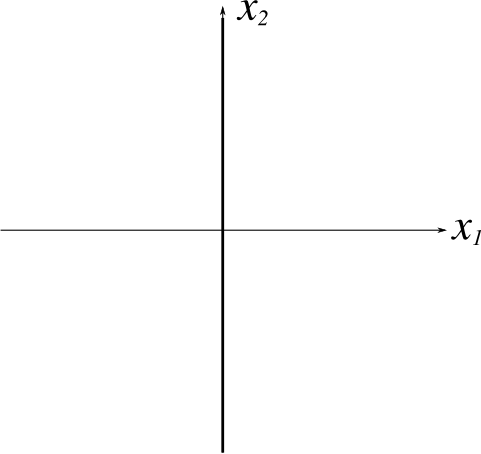
\includegraphics[width=.4\textwidth]{images/08verticalEq}
	\caption{Trajectories.}
	\label{fig:08verticalEq}
\end{figure}

Since $\dot{V}=-x_1^2$ then as long as $x_1\neq0$ the system will keep losing energy so there exists damping of some kind.

By the Barbashin-Krasovskii theorem that we will see later in the course we have that $\dot{V}=0\Rightarrow x_1\to0$ which is better than neutral stability. $x_1=0$ means $x_2$ will go to a constant value and since $x_1\to0$ then $\dot{x}_1\to0$ so $x_2^3\to0\Rightarrow x_2\to0$. This leads to $x_1\to0$ and $x_2\to0$ implying g.a.s.
$\lozenge$
\end{example}

\begin{example}
Consider the system
\begin{align}
\label{eq:lec08ex3}
\dot{x}_1 &= -x_1 + x_1x_2^3 \\
\label{eq:lec08ex4}
\dot{x}_2 &= -x_1^2
\end{align}
The $x_2$-axis is the equilibria manifold. Just looking at the origin we can use the Lyapunov function
\begin{align*}
V &= \tfrac{1}{2}x_1^2 + \tfrac{1}{4}x_2^4 \\
\dot{V} &= x_1(-x_1+x_1x_2^3) + x_2^3(-x_1^2) = -x_1^2 \leq 0
\end{align*}
This means that the origin $x=0$ is stable and the trajectories  are vertical at $x_2=1$ since $\dot{x}_1=-x_1+x_1\cdot 1^3 = 0$ as seen in Figure \ref{fig:08trajectories}. Later in the course we will learn that all the equilibria at $x_2>1$ are unstable and the equilibria at $x_2\leq1$ are g.a.s. That is why the points at $x_2>1$ repel and at $x_2<1$ attract.
$\lozenge$
\end{example}

\begin{figure}[ht!]
	\centering
	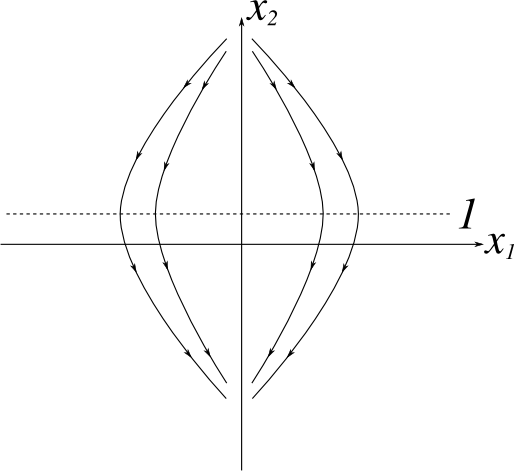
\includegraphics[width=.4\textwidth]{images/08trajectories}
	\caption{Trajectories.}
	\label{fig:08trajectories}
\end{figure}

\section{Terminology}
These terms will be used throughout the rest of the course:
\begin{itemize}
\item \textit{Positive definite}: $V(0)=0$, $V(x)>0\forall x \neq0$.
\item \textit{Positvie semidefinite}: $V(0)=0$, $V(x)\geq0 \forall x \neq0$.
\end{itemize}

Applying these terms to Lyapunov stability theory yields this shorthand notation:
\begin{itemize}
\item $V$ pdf + $\dot{V}$ nsdf $\to$ s
\item $V$ pdf + $\dot{V}$ ndf $\to$ a.s.
\end{itemize}

\section{Lyapunov Level Sets}
For $V(x)=c$ a \textit{level set} is the set of all values $x$ that result in $V(x)=c$. Level sets are circles or ellipses for quadratic functions as illustrated by Figure \ref{fig:08levelSets}. When
\begin{align*}
\dot{V} = \frac{\partial V}{\partial x}f<0
\end{align*}
it means that the inner product always points inward on the level set.

\begin{figure}[ht!]
	\centering
	\includegraphics[width=.4\textwidth]{images/08levelSets}
	\caption{Trajectories.}
	\label{fig:08levelSets}
\end{figure}

%%%%%%%%%%%%%%%%%%%%%%%%%%%%%%%%%%%%%%%%%%%%%%%%%%%%%%%%%%%%%
